%!TEX root = top.tex
\section{Introduction}

\begin{figure} 
  \centering          
  %\begin{tabular}{c}
   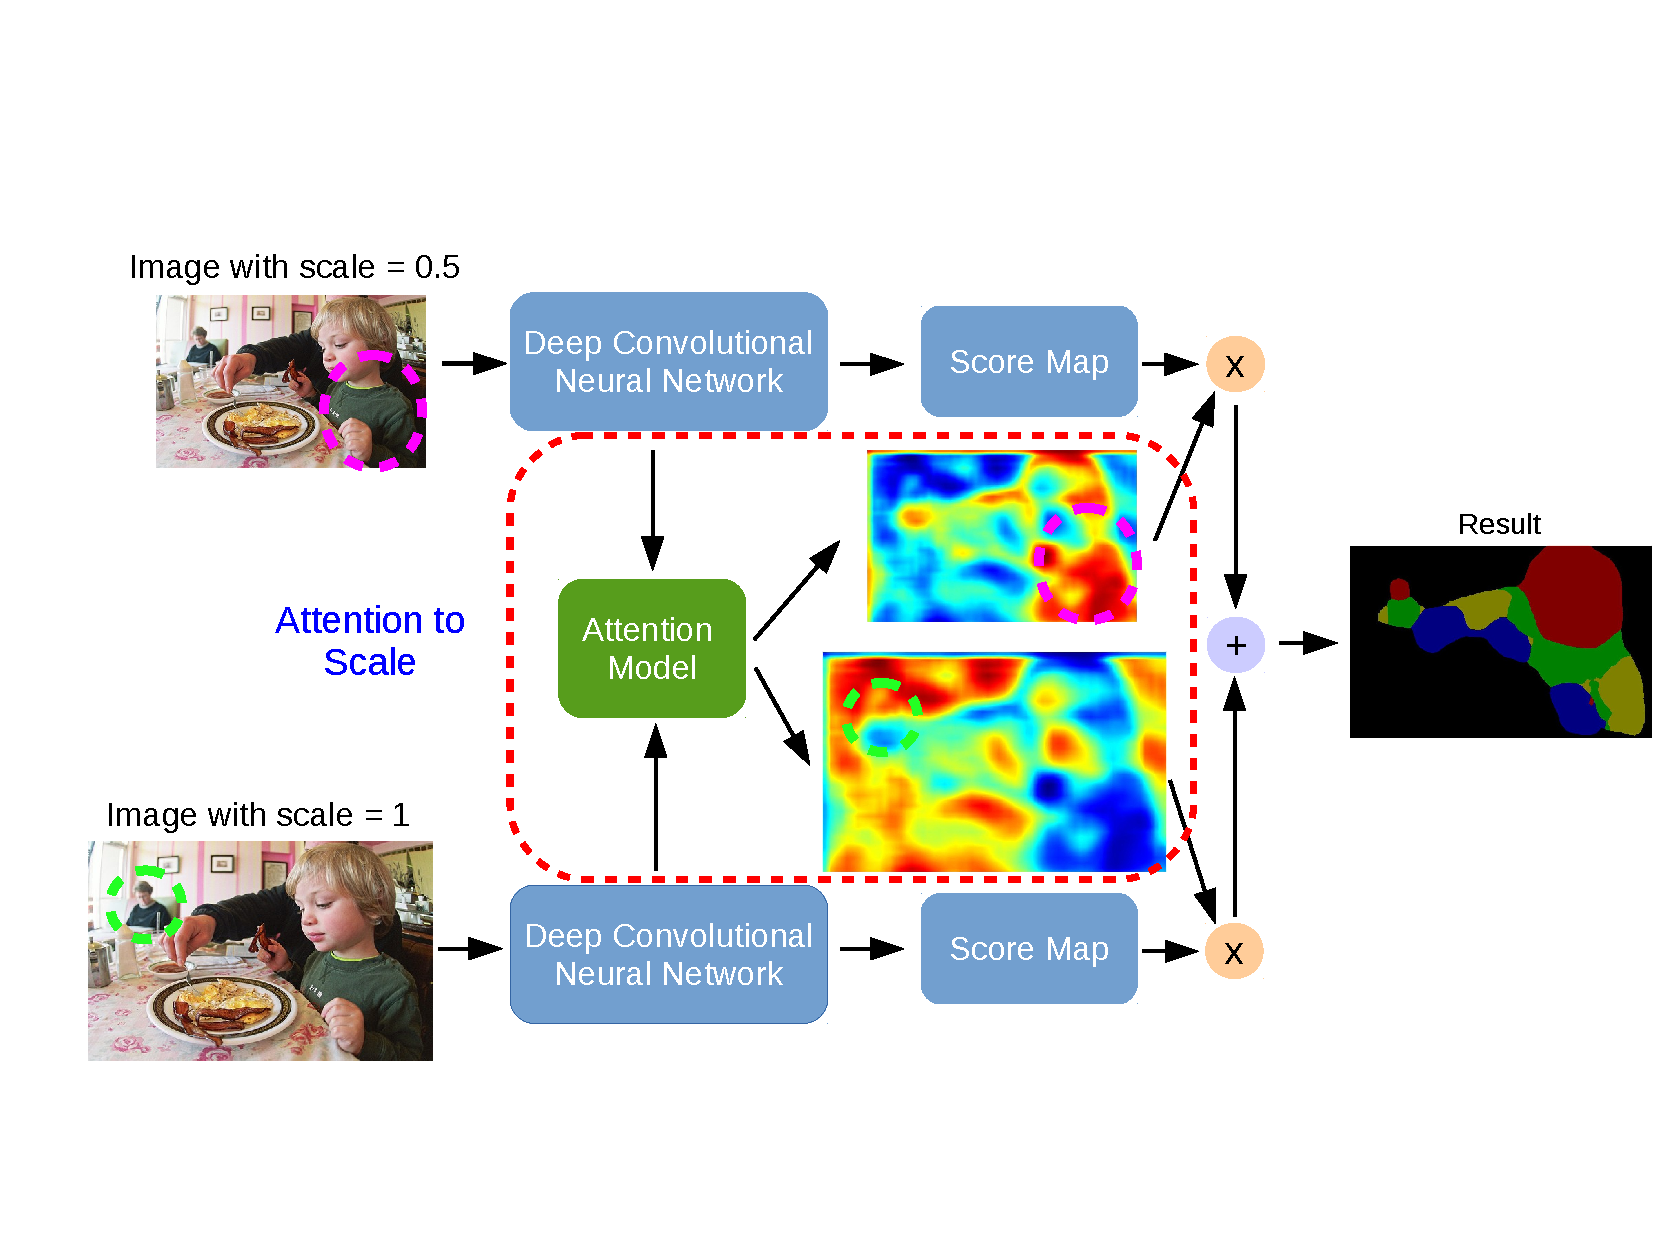
\includegraphics[width=0.99\linewidth]{fig/model_illustration3.pdf} \\
  %\end{tabular}
  \vspace{1pt}
  \caption{Model illustration. The attention model learns to put different weights on objects of different scales. For example, our model learns to put large weights on the small-scale person (green dashed circle) for features from scale = 1, and large weights on the large-scale child (magenta dashed circle) for features from scale = 0.5. We jointly train the network component and the attention model.}
  \label{fig:model_illustration}
\end{figure}  

Semantic image segmentation, also known as image labeling or scene parsing, relates to the problem of assigning semantic labels (\eg, ``person'' or ``dog'') to every pixel in the image. It is a very challenging task in computer vision and one of the most crucial steps towards scene understanding \cite{everingham2014pascal}. Successful image segmentation techniques could facilitate a large group of applications such as image editing \cite{evening2005adobe}, augmented reality \cite{azuma1997survey} and self-driving vehicles \cite{fritsch2013new}.

Recently, various methods  \cite{chen2014semantic, dai2015boxsup, liu2015semantic, noh2015learning, zheng2015conditional, lin2015efficient} based on {\it Fully Convolutional Networks} (FCNs) \cite{long2014fully} demonstrate astonishing results on several semantic segmentation benchmarks. Among these models, one of the key elements to successful semantic segmentation is the use of multi-scale features \cite{farabet2013learning, pinheiro2013recurrent, hariharan2014hypercolumns, long2014fully, mostajabi2014feedforward, lin2015efficient}. In the FCNs setting, there are mainly two types of network structures that exploit multi-scale features \cite{xie2015holistically}. 

The first type, which we refer to as {\it skip-net}, combines features from the intermediate layers of FCNs \cite{hariharan2014hypercolumns, long2014fully, mostajabi2014feedforward, chen2014semantic}.  Features within a skip-net are multi-scale in nature due to the increasingly large receptive field sizes. During training, a skip-net usually employs a two-step process \cite{hariharan2014hypercolumns, long2014fully, mostajabi2014feedforward, chen2014semantic}, where it first trains the deep network backbone and then fixes or slightly fine-tunes during multi-scale feature extraction. The problem with this strategy is that the training process is not ideal (\ie, classifier training and feature-extraction are separate) and the training time is usually long (\eg, three to five days \cite{long2014fully}).

The second type, which we refer to as {\it share-net}, resizes the input image to several scales and passes each through a shared deep network. It then computes the final prediction based on the fusion of the resulting multi-scale features \cite{farabet2013learning, lin2015efficient}. A share-net does not need the two-step training process mentioned above. It usually employs average- or max-pooling over scales \cite{felzenszwalb2010object, ciresan2012multi, papandreou2014untangling, dai2015boxsup}. Features at each scale are either equally important or sparsely selected.

Recently, attention models have shown great success in several computer vision and natural language processing tasks \cite{bahdanau2014neural, mnih2014recurrent, xu2015show, chen2015abc}. Rather than compressing an entire image or sequence into a static representation, attention allows the model to focus on the most relevant features as needed. 
In this work, we incorporate an attention model for semantic image segmentation.
Unlike previous work that employs attention models in the 2D spatial and/or temporal dimension \cite{sharma2015action, yao2015describing}, we explore its effect in the scale dimension.

In particular, we adapt a state-of-the-art semantic segmentation model \cite{chen2014semantic} to a share-net and employ a soft attention model \cite{bahdanau2014neural} to generalize average- and max-pooling over scales, as shown in \figref{fig:model_illustration}. 
%To the best of our knowledge, no other published work explores attention in this dimension.
%In the experiments, we adapt a state-of-art semantic segmentation model \cite{chen2014semantic} to a share-net and incorporate an attention model to it. 
The proposed attention model learns to weight the multi-scale features according to the object scales presented in the image (\eg, the model learns to put large weights on features at coarse scale for large objects). 
For each scale, the attention model outputs a {\it weight map} which weights features pixel by pixel, and the weighted sum of FCN-produced score maps across all scales is then used for classification. %For each scale, the attention model outputs a {\it weight map} which weights the accordingly features pixel by pixel, and from which we are able to visualize the importance of features at different positions and different scales. 
%The weighted sum of FCN-produced score maps across all scales is then used for classification. 

%While all previous works focus on 2D spatial and temporal dimension, we study the effect on the scale dimension which is not addressed in the computer vision literature before.
%The concept of scale here is an encoding of both object depth and semantic scale, corresponding to the weighted selection of feature pyramids that best recognizes objects at different scales.
%The idea behind this is that to recognize objects at different scales, CNN image receptive field size should vary at different pixel locations.
%The observation behind is that human changes pupil focal length when looking at different objects.
%The key contribution of this paper is the scale-attention model for semantic image segmenation, which seems not been addressed in the computer vision literature before.
%The proposed attention model is no more complicated than the fully-convolutional models and is able to utilize multi-scale image features efficiently.
%To the best of our knowledge, no other published work explores attention in this dimension.

%Investigations reveal that one of the key elements of successful semantic segmentation models is the use of multi-scale features \cite{farabet2013learning, pinheiro2013recurrent, hariharan2014hypercolumns, long2014fully, mostajabi2014feedforward, lin2015efficient}. For semantic segmentation, there are mainly two successful types of networks that exploit multi-scale features \cite{xie2015holistically}. The first type, which we refer to as {\it skip-net}, combines features from the intermediate layers of Deep Convolutional Neural Networks (DCNNs) \cite{hariharan2014hypercolumns, long2014fully, mostajabi2014feedforward, chen2014semantic}.  Features within a skip-net are multi-scale in nature due to the increasingly larger receptive field sizes. The second type, which we refer to as {\it share-net}, feeds multi-scale inputs (\ie, resize the input image to several scales) to a shared network and later merge the network outputs. \cite{farabet2013learning, lin2015efficient}. 

%A skip-net usually employs a two-step training process \cite{hariharan2014hypercolumns, long2014fully, mostajabi2014feedforward, chen2014semantic}, where it first trains the deep network backbone and then fixes or slightly fine-tunes during multi-scale feature extraction. The problem with this strategy is that the training process is not ideal (\ie, classifier training and feature-extraction are separate) and the training time is usually long (\eg, three to five days \cite{long2014fully}). 
% For skip-net, a two-step training process is usually employed \cite{hariharan2014hypercolumns, long2014fully, mostajabi2014feedforward, chen2014semantic}. That is, the deep network backbone is firstly trained and then fixed or slightly fine-tuned during multi-scale feature extraction. The problem with this strategy is that the training process is not ideal (\ie, classifier training and feature-extraction are separate) and the training time is usually long (\eg, three to five days \cite{long2014fully}). 

%% For skip-net, a two-step training process is usually employed. There are two cases to perform the two-step training process in the literature. In the first case, the deep network backbone is firstly trained and is fixed during multi-scale feature extraction \cite{hariharan2014hypercolumns, mostajabi2014feedforward, chen2014semantic}. In the second case, a network that produces coarse outputs is firstly trained and is used as initial values to gradually obtain finer results. The problem with the first case is that the training process is not ideal (\ie, classifier training and feature-extraction are separate), while the problem with the second case is that the training time is usually long (\eg, three to five days \cite{long2014fully}). 

%On the contrary, a share-net usually resizes the input image to several scales and passes each through a shared deep network. It then computes the final prediction based on the fusion of the resulting multi-scale features \cite{farabet2013learning, lin2015efficient}. A share-net does not need the two-step training process as mentioned above. It usually employs average- and max-pooling over scales \cite{felzenszwalb2010object, ciresan2012multi, papandreou2014untangling, dai2015boxsup}. In this work, we propose to generalize average- and max-pooling. Our method not only yields better performance over baselines but also allows us to visualize which feature at which scale contributes to the classification most.
%For share-net, the input image is resized to several scales and each is passed through a shared deep network. The final prediction is then based on the fusion of the resulting multi-scale features \cite{farabet2013learning, lin2015efficient}. Share-net does not need the two-step training process mentioned above. average- and max-pooling over scales are usually employed \cite{felzenszwalb2010object, ciresan2012multi, papandreou2014untangling, dai2015boxsup}. In this work, we propose to generalize average- and max-pooling. Our method not only yields better performance over baselines but also allows us to visualize which feature at which scale contributes to the classification most.

%In particular, we employ an attention model \cite{bahdanau2014neural} to generalize average- and max-pooling over scales, as shown in \figref{fig:model_illustration}. The proposed attention model learns to weight the multi-scale features according to the object scales presented in the image (\eg, the model learns to put large weights on features at coarse scale for large objects). In the experiments, we explore a state-of-art semantic segmentation model \cite{chen2014semantic}. We adapt it to a type of share-net and incorporate an attention model to it. We jointly train the attention model as well as the DCNN component. For each scale, the attention model outputs a {\it weight map} which weights the accordingly features pixel by pixel, and from which we are able to visualize the importance of features at different positions and different scales. The weighted sum of DCNN-produced score maps across all scales is then used for classification. 
%In particular, we employ an attention model \cite{bahdanau2014neural} to generalize average- and max-pooling over scales, as shown in \figref{fig:model_illustration}. The proposed attention model learns to weight the multi-scale features according to the object scales presented in the image (\eg, the model learns to put large weights on features at coarse scale for large objects). In the experiments, we explore a state-of-art semantic segmentation model \cite{chen2014semantic}. We adapt it to be a type of share-net and incorporate an attention model to it. The attention model as well as the DCNN component is jointly trained. For each scale, the attention model outputs a {\it weight map} which weights the accordingly features pixel-by-pixel, and by which we are able to visualize the importance of features at different positions and different scales. The weighted sum of DCNN-produced score maps from each scale is then used for classification. 

Motivated by \cite{bengio2007greedy, lee2014deeply, szegedy2014going, xie2015holistically}, we further introduce extra supervision to the output of FCNs at each scale, which we find essential for a better performance. We jointly train the attention model and the multi-scale networks. We demonstrate the effectiveness of our model on several challenging datasets, including PASCAL-Person-Part \cite{chen_cvpr14}, PASCAL VOC 2012 \cite{everingham2014pascal}, and a
subset of MS-COCO 2014 \cite{lin2014microsoft}. Experimental results show that our proposed method consistently improves over strong baselines. The attention component also gives a non-trivial improvement over average- and max-pooling methods. More importantly, the proposed attention model provides diagnostic visualization, unveiling the black box network operation by visualizing the importance of features at each scale for every image position.

%Moreover, we demonstrate that our model generalizes well to other datasets by applying our model trained on PASCAL-Person-Part to some videos from MPII Human Pose dataset \cite{andriluka14cvpr}.

%The proposed model significantly improves over baseline DeepLab-LargeFOV on PASCAL VOC 2012 (6.4\% on test set), and yields significantly better performance than DeepLab-MSc variants (4.5\% on test set) while it only requires one-step {\it end-to-end} training. It also gives non-trivial 1\% improvement over average- and max-pooling methods. More importantly, the proposed attention model provides diagnostic visualization, unveiling the black box network operation by visualizing importance of features at each scale for every image position.

%In short, the improvement of the proposed model is {\it accumulated} by (1) multi-scale inputs (2) attention model (3) extra supervision. The proposed model significantly improves over baseline DeepLab-LargeFOV on PASCAL VOC 2012 (6.4\% on test set), and yields significantly better performance than DeepLab-MSc variants (4.5\% on test set) while it only requires one-step {\it end-to-end} training. It also gives non-trivial 1\% improvement over average- and max-pooling methods. More importantly, the proposed attention model provides diagnostic visualization, unveiling the black box network operation by visualizing importance of features at each scale for every image position.

%% The proposed attention model is embedded within a FCN and is jointly trained end-to-end. For each scale, the attention model outputs a salience map \cite{itti1998model} which will weight the accordingly features pixel-by-pixel. The weighted sum of score maps from each scale is then used for classification. The proposed model is illustrated in \figref{fig:model_illustration}. Particularly, our model is built upon the DeepLab model \cite{chen2014semantic}. We demonstrate the effectiveness of our proposed model on three challenging datasets, including PASCAL-Person-Part \cite{chen_cvpr14}, PASCAL VOC 2012 \cite{everingham2014pascal}, and a subset of MS-COCO 2014 \cite{lin2014microsoft}. The experimental results show that our proposed methods consistently improve over the original DeepLab model.

